


\chapter{Context-free grammars}

There is an entire industry of research based on describing what languages 
can come from which grammars and vice-versa.  Its study is today a mixture 
of computer science, algebra, and linguistics.  In those studies one can 
find a rigorous description of grammars and languages along with what 
computational power is needed to  accept a string.  We have already hinted 
at this complication by indicating that we restrict our thoughts to primitive 
recursions so that the process of parsing comes to an end.

\section{Context sensitive grammar}

Now that we have seen a grammar given by production rules we can explain 
in what way context-free grammars are ``context-free'', and how they 
come to parse as trees.  Consider the situation discussing square-roots 
of natural numbers.
\begin{center}
\begin{Gcode}[]
+<Root> ::= + sqrt(<Nat>)
-<Root> ::= - sqrt(<Nat>)
\end{Gcode}
\end{center}
In this case \code{sqrt{2}:<Root>}.  However, we do not know if this 
was meant as the positive or negative root.  That information 
was left to the surrounding context in which the term was parsed.  
This is a very useful situation as often in algebra we do want to 
speak within a context.  Yet because of the ambiguity if we 
introduce a root in this way and then seek to eliminate we 
cannot be certain of many possible paths got us here.

Meanwhile 
to make this context-free grammar we could use 
\begin{center}
\begin{Gcode}[]
<Root> ::= + sqrt(<Nat>)
         | - sqrt(<Nat>)
\end{Gcode}
\end{center}
Now \code{+sqrt(2):<Root>} and \code{-sqrt(2):<Root>} but 
this grammar rejects \code{sqrt(2)}.  The grammar is less forgiving 
but more precise in the content it now holds for us.

\begin{definition}
    A \emph{context-free grammar} is a grammar whose non-constant 
    production rules are defined on the left of the astonished Walrus 
    \code{::=}.
\end{definition}

\begin{remark}
    The symbols \lstinline{::=}, \lstinline{<Token>} and \lstinline{|} are 
    Backus-Naur Form (BNF) notation, which is popular 
    in computer science.  It is actually subject to its own gammar, admittedly 
    basic and fixed in length.  But you can be forgiven for wondering if this is 
    all circular reasoning.  When this occurs, mathematicians like to attach 
    the word \emph{meta}, which means literally ``self-referential''.
    So BNF would be called a \emph{meta-language}. Sometimes self-referential 
    can be turned into paradoxes (Russell's paradox, G\"odel's Incompleteness,
    Turing's Halting problem).  So you may worry.  But I suppose if you 
    didn't believe in language, why would you be reading?\\
\end{remark}


In mathematics two paths to the same place are said to be a relation.  So
systems that have no cycles, i.e.\ trees, are free of relations, or simply
\emph{free}.  In time we will come to see that every algebraic structure can be
constructed from a free structure with the possible addition of relations.

\begin{remark}{}
    Having two formulas that reduce to the same value is not the same 
as a relation in the grammar.  So what is free in this case 
is the grammar we used for arithmetic formulas.  
For example $7(7+3)(7+3)$ renders the same result 700, and nearly 
by the same steps.  Yet, if we diagrammed that formula as a
parse tree it would quite different
\begin{center}
    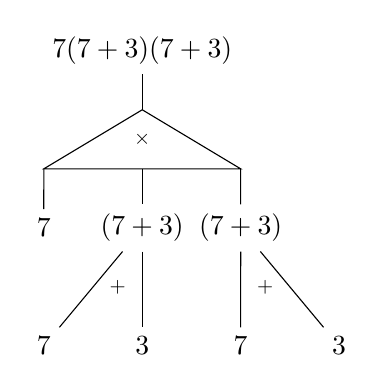
\begin{tikzpicture}[xscale=1.25,yscale=0.75]
        \node (t) at (0,1) {$7(7+3)(7+3)$};
        \node (a) at (-1,-2) {$7$};
        \node (b) at (0,-2) {$(7+3)$}; 
        \node (c) at (1,-2) {$(7+3)$};
        \node (e) at (-1,-4) {$7$};
        \node (f) at ( 0,-4) {$3$};
        \node (g) at ( 1,-4) {$7$};
        \node (h) at ( 2,-4) {$3$};

        \draw (0,0) -- (-1,-1) -- (1,-1) -- cycle;

        \node[scale=0.75] at (0,-0.5) {$\times$};
        \node[scale=0.75] at (-0.25,-3) {$+$};
        \node[scale=0.75] at ( 1.25,-3) {$+$};

        \draw[-] (t) -- (0,0);
        \draw[-] (-1,-1) -- (a);
        \draw[-] (0,-1) -- (b);
        \draw[-] (1,-1) -- (c);
        \draw[-] (b) -- (e);
        \draw[-] (b) -- (f);
        \draw[-] (c) -- (g);
        \draw[-] (c) -- (h);
    \end{tikzpicture}    
\end{center}    
In particular we have not even expressed this as a pair of products 
we have asked instead for a function that takes products of three 
numbers at once.  The ambiguity of how we might achieve this is hidden in the 
triangle \emph{operad} labeled $\times$.
\end{remark}

\section{Formulas: The Free algebra}

There is an evolving pattern in how we described a grammar first for strings, 
then Boolean algebras, and now polynomials.  They each rely on some 
constants set aside at the start.  They also allow for a separate sort for
variables.  Add a final sort for operators and we can describe all the formulas 
we expect in such an algebra.

Now let us notice the pattern.  Our Boolean algebra and our polynomial algebra each 
came in certain form.
\begin{Gcode}[]
    <Formulas<Var>> ::= <Var>
            | <Constants>
            | <Operators>
\end{Gcode}
In fact we can separate operators into order based on how many terms they depend on,
the \emph{valence}, equivalently the degree of the eventual parse tree should that 
production be found in a string.  Letting constants qualify as null-valent operators 
then we have the structure:
\begin{Gcode}[]
    <Formulas<Var>> ::= <Var>
            | <nullvalent operators>
            | <univalent operators>
            | <bivalent operators>
            ...
\end{Gcode}
Or we may abstract in the coarser direction and observe simply the structure operators:
\begin{Gcode}[]
    <Formulas<Var>> ::= <Var>
                      | <Operators>
\end{Gcode}

\begin{definition}
    A \emph{signature} $\sigma$ of an algebra is an (unambiguous) context-free grammar 
    whose production rules are called \emph{operator signatures}.

    A formula with signature $\sigma$ with variables in an alphabet $X$
    is a string accepted by the grammar:
    \begin{Gcode}[]
        <$F_{\sigma}$<X>> ::= <X> | <$\sigma$>
    \end{Gcode}
\end{definition}


\begin{definition}
    A \emph{free algebra} $F_{\sigma}\langle X\rangle$ 
    of a fixed signature $\sigma$ and variables $X$
    is the language accepted 
    \begin{Gcode}[]
        <$F_{\sigma}$<X>> ::= <X> | <$\sigma$>
    \end{Gcode}
    That is, the well-formed formulas with variables $X$.
\end{definition}